\documentclass[conference]{IEEEtran}
\usepackage{graphicx}
\usepackage{eurosym}
\usepackage{amsmath}
\usepackage{amsfonts}
\usepackage{amssymb}
\usepackage{graphicx}
\usepackage{subcaption}
\usepackage{comment}
\usepackage{todonotes}
\usepackage{tikz}
\usepackage{balance}
\usepackage{cite}
\usepackage{lmodern}
\usepackage{lipsum}
\usepackage{hyperref}
\usepackage{tabularx}
\usepackage{fixltx2e}
\usepackage{booktabs}

\renewcommand{\textfraction}{0.15}
\renewcommand{\topfraction}{0.8}
\renewcommand{\bottomfraction}{0.8}
\begin{document}

\title{A Multi--Scale Energy Demand Model suggesting Direct Market Participation of Intelligent Agents}
%Determining Market Participation for Intelligent Agent Groups using Synthetic Multi-Scale Energy Demand Profiles and Time-Shiftable Processes
% author names and affiliations
% use a multiple column layout for up to three different
% affiliations
\author{Review Version submitted at IAT 2015.%\IEEEauthorblockN{Georgios Methenitis, Michael Kaisers, Han La Poutr\'e
}
% \IEEEauthorblockA{Intelligent Systems Group (IS)\\ Centrum Wiskunde \& Informatica\\ Amsterdam, The Netherlands\\ Emails: $\lbrace$Georgios.Methenitis, Michael.Kaisers, Han.La.Poutre$\rbrace$@cwi.nl}}

\maketitle

\begin{abstract} In this paper, we propose a multi-scale model of energy demand that is consistent with observations at a macro scale. We discuss this model in the context of standard load profiles for (residential) electric loads, and demonstrate its use by studying direct market participation of intelligent agents at different aggregation scales of energy consumption. Next to scale, we investigate the benefits of demand response, more precisely intelligent scheduling of time-shiftable electric processes, and virtual storage intra-day and between days. Results show that the increasing electrification and introduction of flexibilities (electric vehicles, thermal applications, storage etc) is going to make direct market participation viable for smaller groups of consumers. Retailers may anticipate competition by intelligent energy cooperatives that directly participate in wholesale markets for electricity.
\end{abstract}
\IEEEpeerreviewmaketitle

\section{Introduction}
\label{sec:Introduction}

% introduction, slps, non-observability
In today's energy system, the major fraction of electricity is provided to power consumers by utility scale power producers through retail aggregators.
Retailers must procure the power for their costumers whose energy consumption profile is not always observable (e.g., due to high cost of smart-meter roll-outs on-site). Standard load profiles~\cite{jardini2000daily} (SLPs) are derived by electricity distribution system operators for several types of consumers. Typical examples include residential, commercial and industrial. Those SLPs are used by retailers to determine the amount of energy that they must procure in the wholesale energy markets (day-ahead and intraday). Typically, SLPs contain an averaged daily consumption profile for the whole year, treating weekdays, weekends, and holidays in a different manner, based on historic data and the temperature. Distribution system operators (DSOs) are computing these SLPs from measurements, based on the portfolio of end-consumers behind a distribution substation. Power producers sell their energy at the wholesale markets, and are influenced via the retailers by this information to plan the amount of electricity they will need to make available at any given time of the (next) day. The goal of a retailer is to minimize the daily imbalances of the network, which can be achieved more cost-efficiently in the day-ahead market than in the intraday market~\cite{kirschen2003demand}. %Individual end-consumers are treated the same based on their averaged load profile $\hat{q}$ of their type of consumption by the DSOs. 

% smart-meters
While computing the average load profile per type of end-consumer is enough to plan over a highly populated portfolio of costumers, this is not the case when a smaller number of end-consumers is considered. Smart--meters are electronic devices that record consumption of electric energy in small intervals of at most an hour and communicate that information at least daily back to the central system for monitoring and billing~\cite{depuru2011smart}. Unlike home energy monitors, smart--meters can gather data for remote reporting, e.g. to replace standard load profiles of consumer types by actual load profile date in future energy markets. Communication between end-user meters and DSOs enables smart power management --- the smart grid. For instance, based on the information of smart--meters intelligent household systems can shift, store or curtail unnecessary loads in a household when imbalances of the network are high.

% First contribution decomposition of SLPs
In this paper we propose a multi-scale model that captures the specific volatility and flexibility in energy demand profiles, while maintaining that the aggregate behavior is consistent with observations at a macro scale (e.g., SLPs in electricity networks). We introduce a method to derive a process aggregation model from a given SLP, which can produce synthetic demand profiles for various scales --- from an individual device to a large city. 

We use the proposed decomposition technique to generate synthetic aggregate demand profiles on several scales. Results from our model show the minimum viable retailer scale for direct participation in the wholesale markets, and how demand response and virtual storage may decrease this minimum scale by one magnitude. Experiments thus address the question under what circumstances (scale, flexibility) intelligent agents should choose a fixed contract with a retailer, or when to become a retailer.

% OUTLOOK
The remainder of this article is organized as follows: Section~\ref{sec:Related} presents related work on modeling electricity demand, Section~\ref{sec:Method} discusses the proposed multi-scale energy demand model and the required parameter derivations to make it consistent with macro observations. Section~\ref{sec:Experiments} illustrates the resulting multi-scale energy demand and demonstrates its use by evaluating direct market participation of agents of various scales and flexibilities. Finally Section~\ref{sec:Conclusion} serves as an epilogue to this work discussing the contributions.


\section{Related Work}
\label{sec:Related}
% problem - previous solutions
The unobservable consumption profiles at lower scales of aggregation, especially single household demand profiles, have given rise to different approaches to model consumption. A semantic approach to household consumption profiles has been studied in related work~\cite{paatero2006model}. Statistics from household data are used to create a bottom-up model, approximating the consumption of a number of devices in hourly intervals. The artificial profiles generated by this model show high correlation with real data.
Another model for the computation of daily electricity and hot-water demand profiles uses the mean appliance and water-tap data, as well as daylight distributions over the yea~\cite{widen2009constructing}. The comparison between generated profiles and the end-user specific electricity measurements in a small sample of households revealed that the generated model preserved the important qualitative features of real data, which was also the case when it was applied at larger scale.

% Our solution
While previous work in the area of generating synthetic consumption data was focussed on building semantic models, we propose a minimalistic but also more universal and versatile process--model. Our model has a different focus: Rather than studying the semantics, the core focus is the multi-scale modeling. Nevertheless, our model could be extended to capture semantic dependencies, e.g.  by joint distributions between the duration and consumption rate of processes. Our approach is a minimal model that can be scaled to any number of processes and can generalize to demand profiles with arbitrary time horizons. The proposed model can generate synthetic load profiles at any scale from a desired expected load profile.

% flexibility
While related work has shown the impact of storage in real-time prices in relation to ramping constraints~\cite{gast2013impact, faghih2011optimal}; based on our model to generate synthetic load profiles, we use flexibility (storage) to study the feasibility of a decreasing the retailer size, in terms of the number of aggregated profiles that are needed to participate directly in the wholesale markets.

% Smart-meter typification
Other work has focused on typifying household load profiles into several categories~\cite{flath2012cluster,hayn2014electricity}. In a decentralized approach, different consumption profile types are important in regards to the possibility of forming groups of complementary types. Their work is thus complementary to ours.

% decentralized demand management
The importance of decentralized approaches for demand side management in the future smart--grid has been shown emphasizing at the improvements of the energy systems needed at the side of consumption~\cite{palensky2011demand}. Consumption loads can be shifted by decentralized demand side management (DSM) in the smart--grid in~\cite{Ramchurn2011a}. Emergent behavior of the agents in a such a scheme alongside with the adaptation to the grid electricity price can result in peak demand reduction.
This has also been studied by formulating an energy consumption scheduling game and analyzing it game theoretically~\cite{Mohsenian-Rad2010}, where agents develop strategies in regards to their daily schedules of their household appliances and loads. Best response strategies from the players resulted in a significant reduction of the peak-to-average of the total electricity demand. Decentralized agent based techniques have also been used to manage micro-storage to allow storage devices in a smart--grid to converge to profitable and efficient behavior~\cite{vytelingum2010agent}. % Coalitional game theory has been used to study cooperative strategies between the self-adapting micro-grids (small parts of the bigger grid) of a distribution network~\cite{saad2011coalitional, saad2012game}, achieving a reduction in electricity transmission losses during simulations. 
While these works focus primarily on the in-depth technology specific aspects of demand response and storage, we will here perform a simplified study of the merits of such technologies, independent of their implementation. Again, our primary parameter of interest is scale, but more precisely we also model storage and demand response by intra-day shifting of flexible demand.

\begin{table}[t]
\small
\centering
\caption{Notation.}
\begin{tabular}{ r c p{0.7\columnwidth} }
\toprule
 Symbol & & Definition \\
\midrule
  $\hat{q}$ & $\triangleq$ & Average load profile\\
  $q_N$ & $\triangleq$ & Synthetic load profile of $N$ processes\\
  $f$ & $\triangleq$ & Process\\
  $k$ & $\triangleq$ & Consumption rate of a process\\
  $\delta$ & $\triangleq$ & Duration of a process\\
  $t_0$ & $\triangleq$ & Starting time of a process\\
  $p_k$ & $\triangleq$ & Probability density function (PDF) of consumption rate\\
  $p_{\delta}$ & $\triangleq$ & PDF of duration\\
  $\bar{P}_{\delta}$ & $\triangleq$ & Complementary cumulative density function (CCDF) of duration\\
  $p_{t_0}$ & $\triangleq$ & PDF of starting time\\
  $N$ & $\triangleq$ & Number of processes\\
\bottomrule
\end{tabular}
\label{tab:notation}
\end{table}

\begin{figure}[b]
\centering
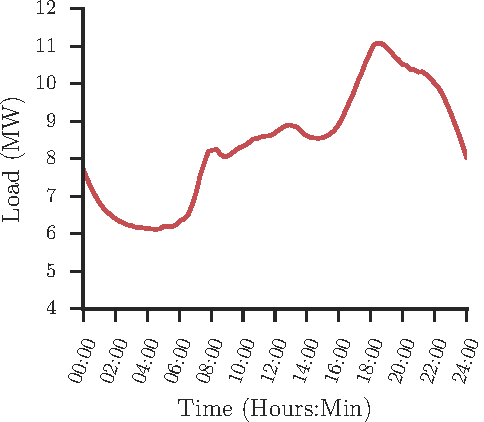
\includegraphics{figures/slp.pdf}
\caption{A typical standard load profile that captures the average household demand at the distribution substation level of aggregation, available as a public dataset~\cite{SLPsource}.}
\label{fig:slp}
\end{figure}



\section{Method}
\label{sec:Method}

% introduction to method
In this section we propose a multi-scale model of energy demand that is consistent with observations at the macro-scale (e.g., standard load profiles for electric demand), and show the necessary parameter derivations. This model aggregates atomic individual \emph{processes}, where the number of processes becomes the \emph{scaling} parameter. The marginal densities of process duration, energy consumption and starting times are tuned to be coherent with macro observations, and the resulting multi-scale model can then generate synthetic data on arbitrary scales.
% Second, we describe how to dynamically form and use cooperative coalitions of agents in a smart--grid based on their synthetic profiles.
Table~\ref{tab:notation} presents the notation that will be used throughout this article.



\subsection{Multi-Scale Model of Energy Demand}\label{sec:LoadProfilesDecomposition}

Figure~\ref{fig:slp} presents the daily load of a distribution substation. We are interested in decomposing such a makro-scale load profile $\hat{q} \in \mathbb{R}^n$, where $n$ is the number of discrete time intervals (the resolution). While the proposed method is general in $n$ and could equally be applied to annual standard load profiles, all experiments and figures use a $24$-hour time horizon with 96 quarter hourly time intervals for a consistent and intuitive presentation of the results.

The load profile decomposition algorithm $lpd()$ generates synthetic load profiles given the desired scaling by the number of processes $N$. 

\subsubsection{Process model}
\begin{figure}[!b]
\centering
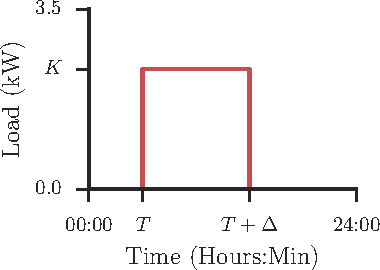
\includegraphics{figures/process.pdf}
\caption{The multi-scale model aggregates over individual atomic \emph{processes}, each characterized by consumption rate $K$ kW, duration $\Delta$, and starting time $T$.}
\label{fig:process}
\end{figure}

Every continuous (non-interrupted) consumption load incurred by a device for some duration can be considered a process.  We define a \emph{process} as the consumption rate $k$ that is taking place, starting at time $t_0$ and having a duration $\delta$. It can then be modeled mathematically as a function $f$:
\begin{equation}
\text{process: }f(t, t_0, \delta, k) =
\left\lbrace
\begin{array}{l}
 k,~t \in [t_0, t_0+\delta)\\
 0, \text{ else}\\
\end{array}
\right.
\end{equation}
Figure~\ref{fig:process} presents a visual representation of the atomic process model that is characterized by consumption $K$ kW, duration $\Delta$, and starting time $T$. The consumption profile of an electric device can consist of a number of processes. A typical household appliance (e.g. TV, heat pump, light bulb, electric vehicle charging, etc.) has several consumption cycles and idle functionality between these cycles, each of its consumption cycles will be treated as a separate process by the discussed model. Varying the number of processes, different aggregation levels of consumption (i.e. a device, a house, or a city) can be approximated. Table~\ref{tab:sizeInter} illustrates different numbers of processes alongside with the interpretation they could have in practice.

\subsubsection{Starting time of process}
A process has been defined as the function $f(t, t_0, \delta, k)$. The synthetic load profile $q_N$ we are interested to generate is given by the following function:
\begin{equation}\label{eq:GenerateSynthetic}
q_N(t, p_{t_0}, p_{\delta}, p_k) = \sum_{i=1}^N f(t, t_0^i, \delta^i, k^i)
\end{equation}
which is the quantity of electricity of $N$ number of processes at timestep $t$. We assume the discrete variables $t_0, \delta, k$ are independent and sampled according to the discrete probability distribution functions $p_{t_0}, p_{\delta}, p_k$ respectively.\footnote{A straight-forward modification allows to treat the variable $k$ as continuous, while making $t_0$ and $\delta$ continuous requires more careful adaptation of the model, which may not have a unique solution in that case.} The expected quantity of $q_N$ is then equal to:
\begin{equation}\label{eq:expectedQuantity}
\mathbb{E}\left[ q_N(t, p_{t_0}, p_{\delta}, p_k) \right] = \sum_{N, T, K} p_{t_0}(T) \bar{P}_{\delta} (t-T) p_k(K) K
\end{equation}
where $\bar{P}_{\delta} = 1 - P_{\delta}$, thus $\bar{P}_{\delta}$ is the complementary cumulative density function (CCDF) of the processes' duration such that: $\bar{P}_{\delta}(t-T) = p_{\delta}(\delta \geq (t-T))$. This corresponds to the expected value of the consumption of a process at $t$ multiplied by the probability that the process started on a specific timestep $T$ and it is still active at timestep $t$ (has duration greater or equal to $t-T$).

\begin{table}[t]
\caption{The energy demand model uses the number of processes as the scaling parameter. Different levels of aggregation correspond to different (ranges of) scales.}
\normalsize\centering\begin{tabular}{ r | l }
\toprule
	Scale & Interpretation \\ 
\midrule
  $10^0 - 10^1$ & Device \\
  $10^1 - 10^2$ & Household \\
  $10^2 - 10^3$ & Apartment building \\
  $10^3 - 10^4$ & Low voltage transformer \\
  $10^5 - 10^6$ & Distribution substation \\
  $10^6 - 10^7$ & City \\
\bottomrule
\end{tabular}
\label{tab:sizeInter}
\end{table}

The interaction of $p_{t_0}, p_{\delta}, p_k$ and $\hat q$ has a unique solution if assumptions are made about three out of the four functions.
Assuming known distributions for the probability density function of a process duration $p_{\delta}$, and the consumption rate of a process $p_k$, we deduce the distribution over starting times from the desired macro profile $\hat q$. As the number of processes is increasing to infinity, the synthetic profile shall converge to the normalized averaged load profile $\hat{q}$:
\begin{equation}\label{eq:approximation_n}
\lim_{N \rightarrow + \infty} \left( \cfrac{q_N(t, p_{t_0}, p_{\delta}, p_k)}{N} \right) \approx \alpha~\hat{q}(t),~\alpha \in \mathbb{R}
\end{equation}
where the normalized per process quantity of an infinite number of processes at timestep $t$ is approximating the quantity of a given standard load profile (see Fig.~\ref{fig:slp}) multiplied by a factor $\alpha$ due to the varying number of processes and the distribution $p_k$. We can normalize the equation further saying that the expectation of $q_N$ is equal to a scaled version of $\hat{q}$: 
\begin{equation}\label{eq:approximation_1}
\mathbb{E}\left[ \cfrac{q_N(t, p_{t_0}, p_{\delta}, p_k)}{N} \right] = \alpha~\hat{q}(t)
\end{equation}
which is the expected quantity per process at timestep $t$. From equations~\eqref{eq:approximation_n},\eqref{eq:approximation_1} the quantity should also approximate the expectation when the number of processes are going towards infinity.
\begin{equation}\label{eq:approximation}
\lim_{N \rightarrow + \infty} \left( \cfrac{q_N(t, p_{t_0}, p_{\delta}, p_k)}{N} \right) \approx \mathbb{E}\left[ \cfrac{q_N(t, p_{t_0}, p_{\delta}, p_k)}{N} \right]
\end{equation}
Using equation~\eqref{eq:expectedQuantity} we can infer the probability density function of $t_0 \in [0, n]$ where $n$ is the time horizon and depends on the chosen resolution for the time axis. We start from the expected value of $q_N$ at timestep $t$, due to independence we can rewrite the equation as:
\begin{equation}
\mathbb{E}\left[ q_N(t, p_{t_0}, p_{\delta}, p_k) \right] = N~\mathbb{E}[k]~\sum_{T} p_{t_0}(T) \bar{P}_{\delta} (t-T)
\end{equation}
replacing the first term according to equation~\eqref{eq:approximation_1} we have:
\begin{align}
\cfrac{\alpha}{N~\mathbb{E}[k]}~\hat{q}(t) &= \sum_{T} p_{t_0}(T) \bar{P}_{\delta} (t-T)\\
\hat{q}'(t) &= \sum_{T} p_{t_0}(T) \bar{P}_{\delta} (t-T) \label{eq:infer_t_0}
\end{align}
where 
\[
q'(t) = \cfrac{\alpha}{N~\mathbb{E}[k]}~\hat{q}(t)
\]
From equation~\eqref{eq:infer_t_0} we can produce a set of linear equations which form the linear system of the form $Ax = b$:
\begin{equation}\label{eq:linearSystem}
\arraycolsep=2pt\def\arraystretch{1.2}
\left[\begin{array}{cccc}  
 \bar{P}_{\delta}(0)  & \bar{P}_{\delta}(n) & \ldots  & \bar{P}_{\delta}(1)\\
 \bar{P}_{\delta}(1)  & \bar{P}_{\delta}(0) & \ldots  & \bar{P}_{\delta}(2)\\
\vdots  & \vdots & \ddots  & \vdots\\
 \bar{P}_{\delta}(n)  & \bar{P}_{\delta}(n-1) & \ldots  & \bar{P}_{\delta}(0)
\end{array}\right]
\times
\left[\begin{array}{c}  
 p_{t_0}(0) \\ 
  p_{t_0}(1) \\
 \vdots \\
 p_{t_0}(n) \\  
\end{array}\right]
=
\left[\begin{array}{c}  
 q'(0) \\ 
  q'(1) \\ 
 \vdots \\
 q'(n) \\  
\end{array}\right]
\end{equation}
Normally matrix $A$ would be a lower triangular matrix, where processes that influence the probability density at timestep $t$ are only the ones starting at timesteps $t_0 \in [0, t]$. In order to model the continuity of our model over the time horizon we assume wrap-around, i.e. processes which start late in the day and have a duration that lasts longer than the day influence the expected quantity at the beginning of the same day (or whatever the horizon of the profile). In this way, matrix $A$ models the past and the future processes that may affect the current probability density function at timestep $t$. Equation~\eqref{eq:infer_t_0} becomes:
\begin{equation}\label{eq:infer_t_0_axis}
\hat{q}'(t) = \sum_{T} p_{t_0}(T) \bar{P}_{\delta} (s)
\end{equation}
where
\begin{equation*}
s =
\left\lbrace
\begin{array}{l}
 t-T~~~~~~~,\forall T \in [0, t]\\
 n-|t-T|,\forall T \in (t, n]\\
\end{array}
\right.
\end{equation*}
For instance, looking at the first row of matrix $A$ that contains the probabilities for every timestep for the duration of a process that starts at timestep $0$, we can infer that the expected quantity for $q$ will be the probability of a process starting at timestep zero and having at least $0$ duration, starting at timestep $1$ and have duration at least $n$, or starting at timestep $n$ and having duration at least $1$. Solving the linear system will result in obtaining the scaled distribution of $p_{t_0}$ due to the scaled quantity $q'$. Normalizing $p_{t_0}$ to sum up to one yields the probability density function of the process starting times.
\begin{figure}[t]
\centering
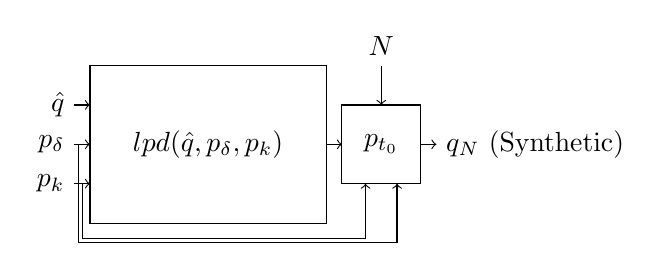
\begin{tikzpicture}
\draw[] (0,0) rectangle (3,2) node[pos=.5] {$lpd(\hat{q}, p_{\delta}, p_{k})$};
\draw[->] (-0.2,1.5) node[anchor=east] {$\hat{q}$} -- (0,1.5) ;
\draw[->] (-0.2,1) node[anchor=east] {$p_{\delta}$} -- (0,1);
\draw[->] (-0.2,0.5) node[anchor=east] {$p_{k}$} -- (0,0.5) ;

\draw[-] (-0.1,0.5)  -- (-0.1,-0.2);
\draw[-] (-0.1,-0.2) -- (3.5,-0.2);
\draw[->] (3.5,-0.2) -- (3.5,0.5);

\draw[-] (-0.15,1)  -- (-0.15,-0.25);
\draw[-] (-0.15,-0.25) -- (3.9,-0.25);
\draw[->] (3.9,-0.25) -- (3.9,0.5);

\draw[->] (3.7,2.0) node[anchor=south] {$N$} -- (3.7,1.5) ;
\draw[->] (3,1) -- (3.2,1) ;
\draw[] (3.2,0.5) rectangle (4.2,1.5) node[pos=.5] {$p_{t_0}$};
\draw[->] (4.2,1) -- (4.4,1) node[anchor=west] {$q_N$ (Synthetic)};
\end{tikzpicture}
\caption{Schematic representation of the \emph{load profile decomposition} algorithm, which derives $p_{t_0}$ from the other marginal densities and the macro scale observations $\hat q$, and subsequent generation of synthetic demand profile $q_N$ on a specific scale $N$.}\label{fig:system}
\end{figure}%

The inferred probabilities $p_{t_0}$ can be used in equation~\eqref{eq:GenerateSynthetic} to generate synthetic load profiles.  Figure~\ref{fig:system} illustrates the described procedure schematically: the decomposition of standard load profiles into a process-model that can be scaled with the tuning of one parameter, the number of processes, approximating different aggregation levels.  

\section{Experiments and Results}
\label{sec:Experiments}

The experimental setup and the results obtained by our experiments are presented in this section. We start by showing the way synthetic data can be generated using the method in the previous section. The resulting load profiles are the basis for retailer scaling experiments, studying the price of electricity in direct market participation under varying assumptions of flexibility.

\begin{figure}[b]
\centering
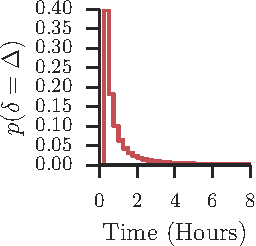
\includegraphics{figures/delta.pdf}~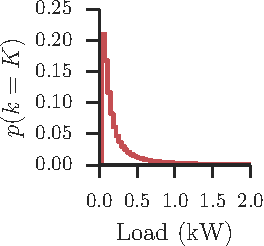
\includegraphics{figures/kappa.pdf}
\caption{Left, probability density function $p_{\delta}$ for the duration (hours) of processes. Right, probability density function $p_k$ over consumption rates (kW) of the processes.}
\label{fig:devide-time-consumption}
\end{figure}

\begin{figure*}[t]
\centering
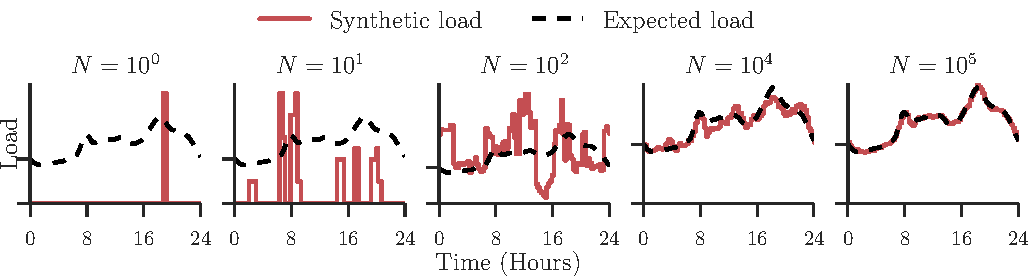
\includegraphics{figures/slps.pdf}
\caption{Example synthetic load profiles generated for different scales (numbers of processes). The kW axis varies between graphs in scale, but the expected quantity is given for comparison. The synthetic profile is approximating the expected value as the number of processes increases.}
\label{fig:art_slps}
\vspace{-0.5cm}
\end{figure*}

\subsection{Multi-Scale Model of Electricity Demand}
\label{sec:Results_Synthetic}

The algorithm, described in detail in Section~\ref{sec:LoadProfilesDecomposition} and Figure~\ref{fig:system}, takes as input the average load profile $\hat{q}$ (see Figure~\ref{fig:slp}), the number of processes $N$ and the probability density functions for the duration and the consumption rate of a process, $p_{\delta} $ and $p_k$ respectively, given in Figure~\ref{fig:devide-time-consumption}. The resulting multi-scale aggregation model of processes is illustrated in Figure~\ref{fig:art_slps}.
All discrete signals used for the quantities described in this section have $96$ values, using four time intervals every hour of the day (quarter hours). The probability density functions $p_{\delta}, p_k, p_{t_0}$ have the same resolution. In general, the model does not put any restrictions on the distributions that can be used. In this experimental setup, we chose independent F-distributions~\cite{winer1971statistical} (heavy tailed distributions) for both probability density functions, based on consumption statistics for household appliances~\cite{zimmermann2012household}.
\begin{align*}
&p_{\delta} = \mathbb{F}(10, 2), \text{ scale = $0.3$}, ~ \delta \in [0.0, 24.0]\\
&p_k = \mathbb{F}(10, 2), \text{ scale = $0.1$},~ k \in [0.0, 3.5]
\end{align*}
Since we are looking into the daily consumption profile of a number of processes, we truncate duration probability function from $0$ to $24$ hours processes to capture the whole margin of a day. The consumption distribution is from zero to $3.5$ kW, given that the maximum electric flow of household connections are $16$A ($230$V).

\begin{figure}[t]
\centering
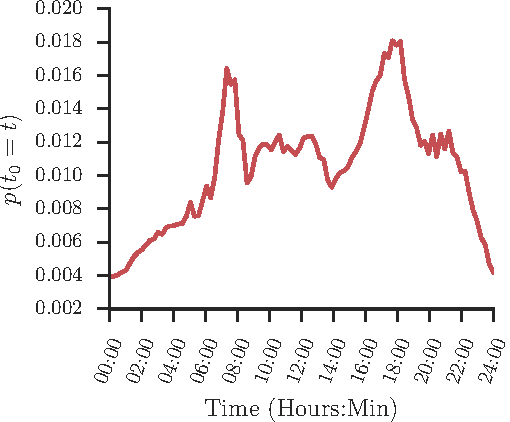
\includegraphics[scale=0.8]{figures/t_0.pdf}
\caption{The probability density function $p_{t_0}$ characterizes the starting times of the processes, and is shown as derived from the standard load profile in Figure~\ref{fig:slp}, and marginal densities in Figure~\ref{fig:devide-time-consumption}. The two peaks at 7am and 5pm match expected activity before and after regular working hours, when demand processes (such as cooking, lights, TV) are initiated.}
\label{fig:distribution_t_0}
\end{figure}

Figure~\ref{fig:devide-time-consumption}, presents the probability density functions for both the consumption rate and the duration of each process. Given the two distributions, the model can be obtained solving the linear system~\eqref{eq:linearSystem}, the result of the linear system of equations when normalized to sum up to unit is the probability density function of the starting time of a process $p_{t_0}$. Figure~\ref{fig:distribution_t_0} illustrates the distribution of probability for the starting time of a process over the day time horizon. Notice that the probability that a process starts is highly increasing after 6 am, and increasing again after 5 pm when people are home and tend to use most of the devices.


\begin{figure}[t!]
\centering
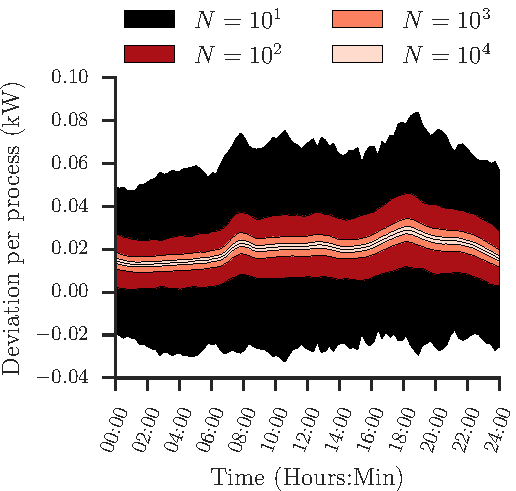
\includegraphics[width=0.9\columnwidth]{figures/std_.pdf}
\caption{Normalized mean plus-minus standard deviation for the expected quantity of electricity, for each number of processes computed from $1000$ generated samples. Consider that all sample profiles are always positive, and actually deviations are skewed.}
\label{fig:Deviation}
\end{figure}


Given the probability density function of the starting time of a device $p_{t_0}$ we can generate synthetic load profiles for specific scales $N$. Recall equation~\eqref{eq:approximation}: as the number of processes increases, the synthetic profile that is obtained should approximate the expected load $\mathbb{E}[q]$. As expected, Figure~\ref{fig:art_slps} shows how using the derived $p_{t_0}$ in equation~\eqref{eq:infer_t_0_axis} indeed gives rise to synthetic profiles that approximate the standard load profile $\hat{q}$ for large $N$. The scaling used in Table~\ref{tab:sizeInter} is used here to illustrate synthetic profiles for different real life scaling scenarios. A single device with expected daily consumption of $2.3$ kWh can be approximated when $N=10^1$. For $N=10^2$ the profile resembles the consumption of a household ($23$ kWh daily consumption). An aggregation of the consumption profiles of several apartments in a building is close to $N=10^3$ ($230$ kWh daily consumption). A low voltage transformer with up to a hundred households corresponds to $N=10^4$. The measurement of the consumption at the substation ($240$ MWh daily load, $N=10^6$) is very close to the expected quantity. In fact, we chose to show a smaller substation scale ($N=10^5$), which already yields very smooth behavior.

\begin{figure}[b]
\centering
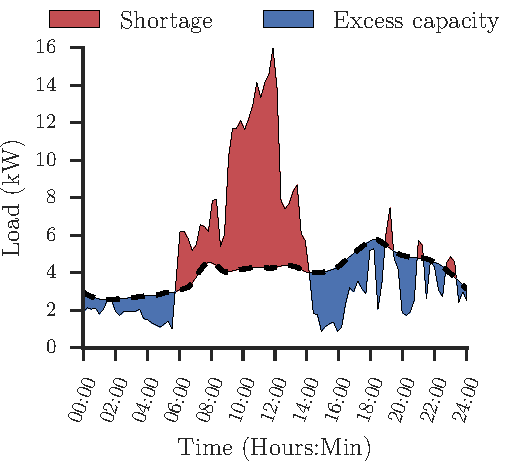
\includegraphics[scale=0.9]{figures/slp_shortage.pdf}
\caption{The dashed line indicates the power profile procured on the day-ahead market. The shaded areas indicate the actual shortage (above) and excess capacity (below). Virtual storage applies a daily netting of shortage and excess, and provides an optimistic bound on any (possibly lossful) storage.}
\label{fig:shortage}
\end{figure}

\begin{figure}[b]
\centering
\vspace{6.4mm}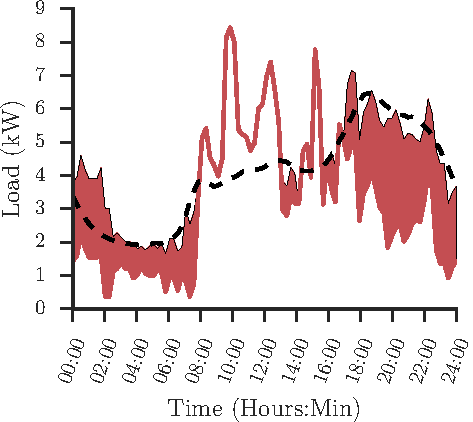
\includegraphics[scale=0.9]{figures/movable.pdf}
\caption{The dashed line indicates the power profile procured on the day-ahead market. The solid line shows power consumed by uncontrollable processes, and the shaded area shows power consumed by time-shiftable processes (demand response), placed with the sequential greedy heuristic.}
\label{fig:movable}
\end{figure}

\begin{figure}[!t]
\centering
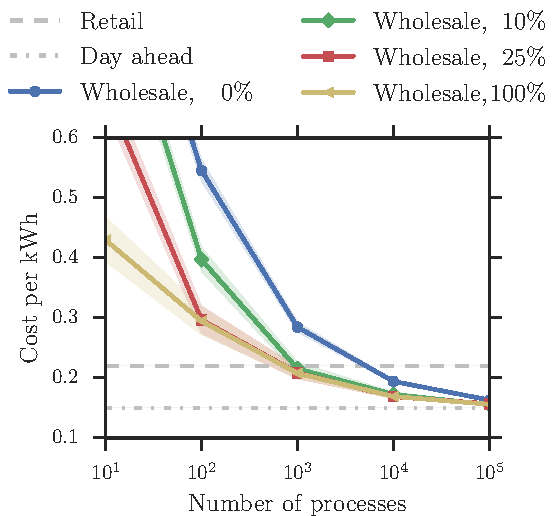
\includegraphics[width=0.9\columnwidth]{figures/Wholesale.pdf}
\caption{Electricity price per kWh (mean of 200 samples and shaded 95 \% confidence interval) for different aggregation scales and four levels of \textbf{virtual storage}. Retailers in the order of $10^4$ processes (ca. 200 households) can already participate directly in the wholesale markets without flexibility, while at least $10 \%$ virtual storage brings costs of direct market participation below retail for smaller collectives (ca. 20 households).}
\label{fig:wholesale}
\end{figure}


As an initial evaluation of the profiles at different scales, % In the day-ahead market electricity aggregators and DSOs are buying the expected quantity of electricity based on the mean quantity of their portfolio of consumers. The imbalances of the intraday consumption of their portfolio will result in higher prices in the intraday market.
Figure~\ref{fig:Deviation} illustrates the standard deviation computed from $1000$ sample synthetic profiles for different numbers of processes. The figure shows the mean and standard deviation normalized per process to obtain same scaling for all profiles. It can be observed that as the number of processes gets larger the standard deviation gets lower, and thus easier to predict. This is the main advantage that larger retailers have for direct wholesale energy market participation. The next section will address an explorative study of market participation on different scales. %resulting to less expected imbalances from the mean in the intraday load profile.

\subsection{Wholesale Market Participation}

The next experiments investigate the scale at which intelligent agents can directly participate in the wholesale market instead of the retail market. In the future smart--grid, small collectives of households may participate as entities in the wholesale market instead of paying flat tariffs for their daily consumption. This would be a vital contribution to tapping into local flexibilities, which are thus far unavailable to the market, since retail customers have no financial incentives to align their behavior with the power grid's needs.
We perform two experiments, studying the price per kWh that retailers can achieve at different scales and with varying flexibility, which is first provided by a virtual battery and second by demand response, more specifically by time-shifting flexible processes. For the retail market, we assume a flat electricity tariff of $0.22$ \euro/kWh. An agent participating in the wholesale markets directly may buy either on the day-ahead market, where prices are more formidable but information is limited to the anticipated expected demand $\hat q$ scaled according to $N$, or on the day itself via balancing markets (in practice either the intraday market or going into imbalance, which is automatically settled by the DSO through reserve markets). We assume a $0.15$ \euro/kWh price for the day-ahead market, adding taxes and surcharges to the trading price but saving the usual retailer profit when directly participating in the market. For the balancing we assume a 10-fold penalty cost ($1.50$ \euro/kWh) for energy that has not been procured on the day-ahead market. Over-procured capacity is wasted without additional cost.

\subsubsection{Virtual Storage}

In this experimental setup flexibility is modeled as the percentage of the daily consumption that can be transferred within the day, resulting in the reduction of imbalances to be procured on the balancing market. As an optimistic scenario (lower bound) of any intra-day flexibility, we assume lossless storage in the form of a daily netting (virtual battery), as illustrated in Figure~\ref{fig:shortage}.

The results are given in Figure~\ref{fig:wholesale}, which presents the price per kWh for four levels of flexibility over various scales. For comparison, the retail and ahead market prices are given. Direct market participation without flexibility is viable from a magnitude of $10^4$ processes, which is the crucial point when an agent can become a retailer on the wholesale market as the price is getting smaller than the flat retail market tariffs. Lossless storage of just $10$ \% would move the minimum viable scale down by a magnitude, with further flexibility having no significant effect.

\subsubsection{Intelligent Demand Response}

We now use a more sophisticated process to model the flexibility induced by demand response in the future smart--grid, illustrated in Figure~\ref{fig:movable}. Demand response is modeled as (a subset of) time-shiftable processes. We use a fraction (e.g., $10\%$) of the total number of processes as processes that can be moved during the day. However, the processes are not know on the day ahead. This corresponds to the assumption that it may be unclear how empty the car battery will be, or how big a laundry needs to be run. Thus, even time-shiftable processes remain stochastic in the two variables of consumption and duration.

Having a number of processes that can start at any time during the day, the agent uses an intelligent (sequential, greedy) heuristic to choose the best starting time that each of them will take. For each time-shiftable process, the starting time that minimizes positive imbalances is chosen sequentially, considering the sum of all uncontrollable and previously placed processes, until all processes are placed one by one. Figure~\ref{fig:movable} presents a consumption profile of $200$ processes from which $40$ of them are movable. Same prices are used in this experimental setup as the ones introduced in the previous experiment. Figure~\ref{fig:wholesale_flex} presents the price per kWh that is obtained at different scales in the wholesale and retail market with or without time-shiftable processes. The non-flexible line is equivalent to the previous experiment, while demand response flexibility is more restricted than the virtual battery due to the continuation of processes. Similar to the previous experiment, flexibility decreases viable market participation scale by a magnitude. However, at least $25$ \% demand response are needed to achieve this result.

\begin{figure}[!t]
\centering
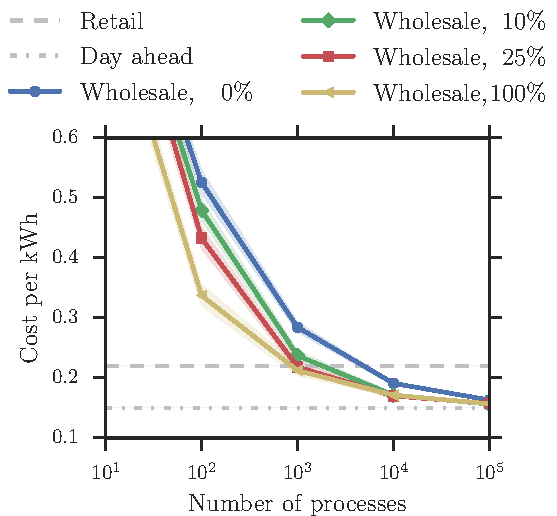
\includegraphics[width=0.9\columnwidth]{figures/Wholesale_flex.pdf}
\caption{Electricity price per kWh (mean of 200 samples and shaded 95 \% confidence interval) for different aggregation scales and four levels of \textbf{demand response} penetration. Above $25 \%$ time-shiftable processes bring costs of direct market participation below retail for smaller collectives (ca. 20 households).}
\label{fig:wholesale_flex}
\end{figure}


The large increase at lower scales is primarily attributed to the unpredictable total energy consumption during the trading horizon of a full day. This implies that demand curtailment, and shifting between consecutive trading days provides a key resource to further decrease the viable scale of direct electricity market participation.

\subsubsection{Between-Day Storage}

While the previous two case studies focused on the benefits of intraday demand response, here we extend the first model of virtual storage by incorporating between-day transfer. We assume each day starts with a reserve capacity (e.g. battery or heat buffer) equal to the flexibility percentage of the actual daily consumption. During the day, shortages of electricity are balanced using demand response (see Figure~\ref{fig:shortage}). In addition, the total energy consumption that day can be curtailed using the between-day storage. Replenishing this storage is planned for the next day with the day-ahead price. While we retain the lossless model for intraday demand response (as a model of time-shifting), the balancing quantity for recharging in the next day is penalized by a loss factor of $30\%$ -- this corresponds to round-trip storage losses in a battery or heat buffer, and increases the quantity bought the next day. Comparable to previous results, Figure~\ref{fig:Wholesale_betweenDay} presents the price per kWh for four different percentages of flexibility and for varying scales. Note that between-day transfer yields high gains despite the losses involved in medium-term storage. If storage capacity exceeds daily consumption, results show that participation in the wholesale market becomes viable for an aggregation level of $100$ processes (a large household), an order of magnitude less than using mere intraday demand response.


\section{Conclusions}
\label{sec:Conclusion}

\begin{figure}[!t]
\centering
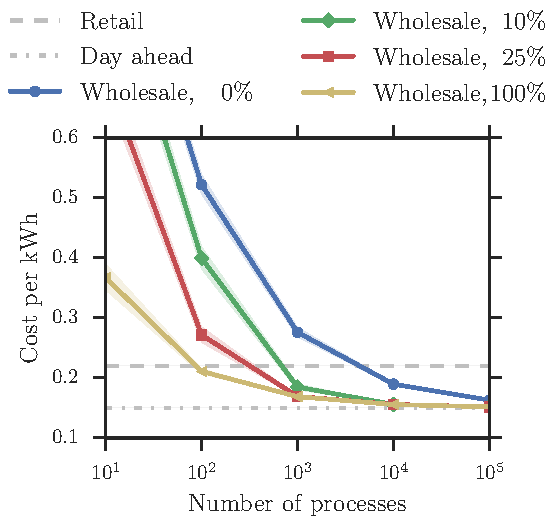
\includegraphics[width=0.9\columnwidth]{figures/Wholesale_betweenDay.pdf}
\caption{Electricity price per kWh for different aggregation scales and four levels of storage capacities. Mean values computed using $200$-independent samples, 95$\%$ confidence interval is shown by the shaded areas.}
\label{fig:Wholesale_betweenDay}
\end{figure}

This article provides primarily two contributions: First, we have introduced a multi-scale energy demand model, aggregating processes, and an algorithm for alignment with given macro observations, such as standard load profiles. %We believe that this model is appropriate to approximate the consumption in a household level, where smart--meter data is difficult to be obtained and used for experimental purposes.
Second, experiments show the business case for participating in the wholesale electricity markets at varying retailer scales, and how flexibility in the form of (virtual) storage and demand response reduces the minimum viable scale. The decrease in costs given sufficient flexibility, especially between-day, may bring the required aggregation scale down to the size of common place existing housing cooperatives, such as large apartment buildings. These cooperatives often already make joint long-term investments into their infrastructure. In combination with increasing flexibilities (electric vehicles, HVAC etc.) and in the context of rising energy prices and future markets with lower participation fees, this may make direct market participation in conjunction with local renewable production a viable future option.

% Limitations
For the sake of clarity and brevity, upfront investment costs and market fees have been neglected, and other simplifying assumptions have been made. First, the duration, power consumption and starting time of processes were treated as independent variables. Second, only one type of atomic process has been used. Third, only one type of (residential) consumption has been approximated. % Finally, the market side was treated heuristically, and optimization on the ahead market opens up various opportunity to build on this model.
% 
% Extensions
The plasticity of our model allows straight-forward extensions to address each of these limitations. These extensions include but are not limited to (1) joint distributions over process characteristics, (2) considering further process types (e.g., recurring cycles), (3) approximating other demand types, supply profiles (e.g., of solar or wind generation), or even other commodities (heat, gas). In addition, the ahead-market has been tackled heuristically and can be optimized to further improve the gains. % In addition, the model can be adapted if the assumptions about known information change, e.g. if the set of controllable processes would be known this can be taken into account by the ahead trading.
The model is therefore more widely applicable to study multi-scale effects of demand and supply aggregation and flexibilities in energy systems.


\bibliographystyle{IEEEtran}
\balance
\bibliography{references}

\end{document}
